\documentclass[../main]{subfiles}
\begin{document}

\Large
\begin{tabu}{clr}
	\multirow{6}{1in}{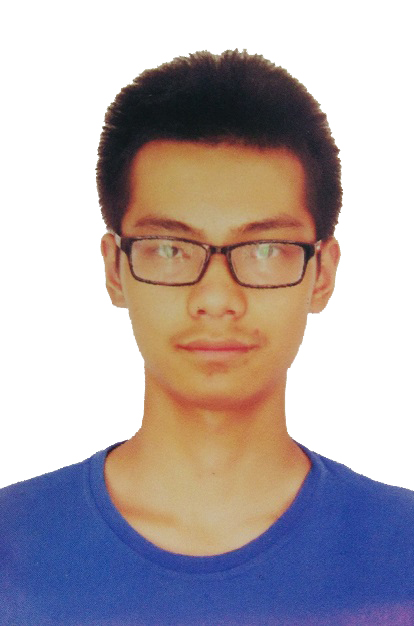
\includegraphics[width=0.88in]{images/profile.jpg}} & \faMale\
	\scshape{吴振宇}                                                         & {\faPython\ Python~}\progressbar{0.95}                                                    \\
	                                                                      & \email{wuzhenyu@ustc.edu}                          & {\faDraftingCompass\
	Perl~}\progressbar{0.8}                                                                                                                                           \\
	                                                                      & \phone{+86~183~555~28308}                          & {\faLinux\ Linux~}\progressbar{0.85} \\
	                                                                      & \faBlog\ \url{https://freed-wu.github.io}          &
	{$\mathcal{C}$\ C~}\progressbar{0.8}                                                                                                                              \\
	                                                                      & \github[Freed-Wu]{https://www.github.com/Freed-Wu} & {\faVimeo\
			Vim~}\progressbar{1}
\end{tabu}
\normalsize

\section{\faGraduationCap\ 教育}%
\label{sec:zh_education}

\datedsubsection{\faUniversity\ \textbf{南京理工大学}}{2016 年 9 月 $\sim$ 2021 年6 月}%
\faGraduationCap\ \emph{学士}\ \faBolt\ 电子信息工程
\datedsubsection{\faUniversity\ \textbf{中国科学技术大学}}{2021 年 9 月 $\sim$ 现在}%
\faGraduationCap\ \emph{学术硕士在读}\ \faBolt\ 信息与通信工程

\section{\faUsers\ 项目经历}%

\datedsubsection{\faCogs\ 航天舱视频回传}{研一}%
载人航天飞船航天舱内部宇航员的视频需要经过压缩后回传到地面。

负责任务:将传统视频编码算法(H264)用 DSP 的汇编语言和 C 语言实现后部署到 DSP 上。\href{https://github.com/Freed-Wu/x264}{代码}

\datedsubsection{\faCogs\ 极端条件视频编码}{研二}%
DSP 上的视频编码算法的 FPS 难以满足较高的实时性,需要通过降采样降低视频分辨率来
提高 FPS。

负责任务:为之前的部署到 DSP 上的视频编码算法(H264)添加一个可选的降采样模块。\href{https://github.com/Freed-Wu/x264-dsp}{代码}

\datedsubsection{\faCogs\ 深空探测图像回传}{研二}%
深空探测器环境恶劣,拍摄的图像难以回传,基于深度学习的图像压缩算法(iWave)比传统的图像压缩
算法能得到更低的码率和失真。

负责任务:将基于深度学习的图像压缩算法(iWave)部署到 SoC 上。

\section{\faUsers\ 科研经历}%
Motivation: 基于深度学习的图像视频编解码的鲁棒性远不如传统算法

Method: 我们通过集成对抗训练,知识蒸馏,随机化的方法提升鲁棒性

Contribution: 我们第一个将集成对抗训练等方法引入到深度学习图像编码中来,使之达
到了能和传统算法相比拟的地步,同时我们保持原有深度学习算法优越的图像编解码能力。

\section{\faCogs\ 技术栈}%

深度学习,模型部署,传统视频编码,嵌入式开发,python,DSP 汇编语言,C,单元测试,CI/CD

\section{\faHeart\ 荣誉}%

\datedline{\faEnvelopeOpenText\ 2019 专利:\href{http://epub.sipo.gov.cn/}{CN109255866A}\ 基于红外传感器的无线控制智能插座}{}
\datedline{\faEnvelopeOpenText\ 2019 专利:\href{http://epub.sipo.gov.cn/}{CN109301609A}\ 非接触式手势门锁装置及实现方式}{}
\datedline{\faThumbsUp\ 2018 国家奖学金,特等奖学金 2019 华为奖学金}{}
\datedline{\faRocket\ 2018 江苏省电子设计竞赛二等奖\ 美国大学生数学建模竞赛二等奖\ 大学生高等数学竞赛一等奖}{}

\end{document}
